\documentclass[aspectratio=169, 10pt]{beamer}

% --- Packages ---
\usepackage[utf8]{inputenc}
\usepackage[T1]{fontenc}
\usepackage{lmodern}
\usepackage{graphicx}
\usepackage{booktabs}
\usepackage{tikz}
\usetikzlibrary{shapes,arrows,positioning,shadows,fit,backgrounds}
\usepackage{amsmath,amssymb}
\usepackage{hyperref}
\usepackage{xcolor}
\usepackage{colortbl}

% Custom symbols for comparison tables
\newcommand{\ok}[1]{{\color{green!60!black}\textbf{\checkmark}\ \scriptsize #1}}
\newcommand{\ko}{{\color{red!70!black}\textbf{$\times$}}}

% --- Custom Theme/Style Definition ---
% Professional & Modern color palette (Deep Navy & Accent Gold/Cyan)
\definecolor{primaryBlue}{HTML}{0A2540}       % Dark professional navy
\definecolor{secondaryBlue}{HTML}{0070F3}     % Vibrant modern blue
\definecolor{accentGold}{HTML}{FFB000}        % Warm highlight gold
\definecolor{textDark}{HTML}{2D3748}          % Clean charcoal text
\definecolor{bgLight}{HTML}{F8FAFC}           % Soft off-white background
\definecolor{cardBg}{HTML}{FFFFFF}            % Pure white for cards/blocks
\definecolor{borderLight}{HTML}{E2E8F0}       % Subtle borders

% Apply global colors
\setbeamercolor{background canvas}{bg=bgLight}
\setbeamercolor{normal text}{fg=textDark}
\setbeamercolor{structure}{fg=primaryBlue}
\setbeamercolor{alerted text}{fg=accentGold}

% Fonts
\usefonttheme{professionalfonts}
\setbeamerfont{title}{size=\LARGE, series=\bfseries}
\setbeamerfont{subtitle}{size=\large, shape=\itshape}
\setbeamerfont{frametitle}{size=\Large, series=\bfseries}
\setbeamerfont{author}{size=\normalsize}
\setbeamerfont{institute}{size=\small}
\setbeamerfont{date}{size=\small}

% Disable navigation symbols
\setbeamertemplate{navigation symbols}{}

% Custom Bullet Points
\setbeamertemplate{itemize items}[circle]
\setbeamercolor{itemize item}{fg=secondaryBlue}
\setbeamercolor{itemize subitem}{fg=primaryBlue}

% Custom Block Styling (Modern Cards)
\setbeamercolor{block title}{bg=primaryBlue, fg=white}
\setbeamercolor{block body}{bg=white, fg=textDark}
\setbeamertemplate{blocks}[rounded][shadow=true]

% Title Page Customization
\setbeamertemplate{title page}{
    \begin{tikzpicture}[remember picture,overlay]
        % Background geometric shapes
        \fill[primaryBlue] (current page.south west) rectangle ([xshift=0.35\paperwidth]current page.north west);
        \path[fill=secondaryBlue, opacity=0.8] (current page.south west) -- ([xshift=0.35\paperwidth]current page.south west) -- ([xshift=0.25\paperwidth]current page.north west) -- cycle;
        
        % Logo placement in top-left
        \node[anchor=north west, xshift=1.2cm, yshift=-0.6cm] at (current page.north west) {
            
\includegraphics[height=1.4cm]{Logo_IIITL.png}
        };
        
        % Title & Subtitle in the main content area (right side)
        \node[anchor=west, text width=0.58\paperwidth, align=left, xshift=0.38\paperwidth, yshift=1.3cm] at (current page.west) {
            \begin{minipage}{\linewidth}
                \flushleft
                % Left accent bar
                \begin{tikzpicture}[baseline=(T.base)]
                    \node(T)[inner sep=0pt, outer sep=0pt, align=left, text width=0.55\paperwidth]{
                        {\color{primaryBlue}\usebeamerfont{title}\inserttitle}\par
                        \ifx\insertsubtitle\@empty\else
                            \vspace{0.25cm}
                            {\color{secondaryBlue!80}\usebeamerfont{subtitle}\insertsubtitle}\par
                        \fi
                    };
                    \draw[secondaryBlue, line width=4pt] ([xshift=-12pt]T.north west) -- ([xshift=-12pt]T.south west);
                \end{tikzpicture}
            \end{minipage}
        };
        
        % Author & Metadata in the main content area (lower right)
        \node[anchor=south west, text width=0.58\paperwidth, align=left, xshift=0.38\paperwidth, yshift=0.9cm] at (current page.south west) {
            {\color{secondaryBlue}\textbf{\usebeamerfont{author}\insertauthor}}\par\vspace{0.15cm}
            {\color{textDark!85}\usebeamerfont{institute}\insertinstitute}\par\vspace{0.35cm}
            {\color{textDark!50}\usebeamerfont{date}\insertdate}
        };
    \end{tikzpicture}
}

% Header (Frametitle) Styling
\setbeamertemplate{frametitle}{
    \nointerlineskip
    \begin{beamercolorbox}[wd=\paperwidth,ht=1.2cm,dp=0.4cm]{}
        \begin{tikzpicture}[remember picture,overlay]
            \fill[primaryBlue] (current page.north west) rectangle ([yshift=-1.2cm]current page.north east);
            \fill[secondaryBlue] (current page.north west) rectangle ([xshift=0.08\paperwidth, yshift=-1.2cm]current page.north west);
            \node[anchor=west, xshift=0.12\paperwidth, yshift=-0.6cm] at (current page.north west) {
                \color{white}\usebeamerfont{frametitle}\insertframetitle
            };
            % Small logo on the right side of headers
            \node[anchor=east, xshift=-0.4cm, yshift=-0.6cm] at (current page.north east) {
                
\includegraphics[height=0.8cm]{Logo_IIITL.png}
            };
        \end{tikzpicture}
    \end{beamercolorbox}
    \vspace{0.3cm}
}

% Footer (Footline) Styling
\setbeamertemplate{footline}{
    \begin{beamercolorbox}[wd=\paperwidth,ht=0.6cm,dp=0.2cm]{}
        \begin{tikzpicture}[remember picture,overlay]
            \fill[primaryBlue!10] (current page.south west) rectangle (current page.south east);
            \draw[secondaryBlue, line width=1.5pt] (current page.south west) -- (current page.south east);
            
            % Left footline: Institution
            \node[anchor=west, xshift=0.5cm, yshift=0.3cm] at (current page.south west) {
                \tiny\color{primaryBlue!80}\insertshortinstitute
            };
            
            % Center footline: Slide Title
            \node[anchor=center, yshift=0.3cm] at (current page.south) {
                \tiny\color{primaryBlue!80}\insertshorttitle
            };
            
            % Right footline: Page Numbers
            \node[anchor=east, xshift=-0.5cm, yshift=0.3cm] at (current page.south east) {
                \tiny\color{primaryBlue!80}\insertframenumber{} / \inserttotalframenumber
            };
        \end{tikzpicture}
    \end{beamercolorbox}
}

% --- Presentation Info ---
\title[Agricultural Expert System]{Toward a Next Generation \\ Agricultural Expert System}
\subtitle{A Multimodal Conversational Approach}
\author[Shajid Ali Khan]{Shajid Ali Khan}
\institute[IIIT Lucknow]{
    \textbf{Supervisor:} Dr. Deepak Kumar Singh \\
    \vspace{0.2cm}
    Department of Computer Science \\
    Indian Institute of Information Technology, Lucknow
}
\date{\today}

% --- Document Content ---
\begin{document}


% Frame 3: Related Work & Research Gaps
\section{Related Work \& Research Gaps}
\begin{frame}{Related Work \& Research Gaps}
    \centering
    \vspace{-0.2cm}
    \renewcommand{\arraystretch}{1.25}
    \resizebox{1.0\textwidth}{!}{
        \begin{tabular}{llcccccccc}
            \toprule
            \textbf{System} & \textbf{Venue} & \shortstack{\textbf{Multi-agent} \\ \textbf{Router}} & \shortstack{\textbf{VLM} \\ \textbf{Disease}} & \shortstack{\textbf{Soil} \\ \textbf{Sensor}} & \shortstack{\textbf{Weather} \\ \textbf{Prediction}} & \shortstack{\textbf{XAI} \\ \textbf{Farmer UI}} & \shortstack{\textbf{Voice /} \\ \textbf{Indic}} & \shortstack{\textbf{Market} \\ \textbf{Price}} & \textbf{Deployed} \\
            \midrule
            Farmer.Chat \cite{farmerchat2024} & ACM 2024 & \ko & \ko\ (Generic) & \ko & \ok{API} & \ko & \ok{Partial} & \ko & \ok{565k users} \\
            AgroAskAI \cite{agroaskai2024} & arXiv 2024 & \ok{Chain} & \ko & \ko & \ok{Dedicated} & \ko & \ok{Partial} & \ko & \ko \\
            AgriGPT \cite{agrigpt2025} & arXiv 2025 & \ok{Data engine} & \ok{VL ext.} & \ko & \ok{Partial} & \ko & \ko & \ko & \ko \\
            AgriM-LLM \cite{agrimllm2026} & Preprints 2026 & \ko & \ok{Best VE} & \ko & \ko & \ko & \ko & \ko & \ko \\
            \rowcolor{secondaryBlue!10} \textbf{AgriDoctor (Base)} \cite{agridoctor2025} & IEEE 2025 & \ok{Router+5} & \ok{Strong} & \ko & \ko & \ko & \ok{CN/EN only} & \ko & \ko \\
            AgriBuddy \cite{agribuddy2025} & BRAC 2025 & \ok{Partial} & \ok{CNN rice} & \ko & \ok{Partial} & \ko & \ko & \ko & \ok{Partial} \\
            PhenoAssistant \cite{phenoassistant2026} & Nature 2026 & \ok{Yes} & \ok{Research} & \ko & \ko & \ko & \ko & \ko & \ko\ (Lab) \\
            Agentic AI \cite{agenticmdpi2026} & MDPI 2026 & \ok{4 agents} & \ok{Rice CNN} & \ok{Partial} & \ok{Dedicated} & \ko & \ko & \ko & \ko \\
            \bottomrule
        \end{tabular}
    }
    \vspace{0.15cm}
    \begin{block}{\footnotesize Key Research Gaps Identified}
        \footnotesize
        \begin{itemize}
            \item \textbf{Soil Sensor Fusion} and \textbf{Market Price} features are completely missing from existing systems.
            \item No prior platform supports explainable AI (\textbf{XAI}) for farmer UIs or comprehensive \textbf{Indic speech} interfaces.
        \end{itemize}
    \end{block}
\end{frame}

\section{Problem Statement}
\begin{frame}{Problem Statement}
    \vspace{0.8cm}
    \setbeamercolor{problemBox}{bg=secondaryBlue!10, fg=textDark}
    \begin{beamercolorbox}[wd=\textwidth, rounded=true, shadow=true, sep=0.4cm]{problemBox}
        Current agricultural AI systems are fatally fragmented: deployed chatbots lack visual diagnostics, advanced vision models lack interactive conversational interfaces, multi-agent setups ignore live market data, and none deliver explainable advice in native Indic languages. Consequently, no existing framework integrates speech, image, soil sensors, weather prediction and live market data into a single trustworthy session.
    \end{beamercolorbox}
\end{frame}


% Frame 7: System Architecture
\section{System Architecture}
\begin{frame}{System Architecture}
    \vspace*{-0.55cm}
    \centering
    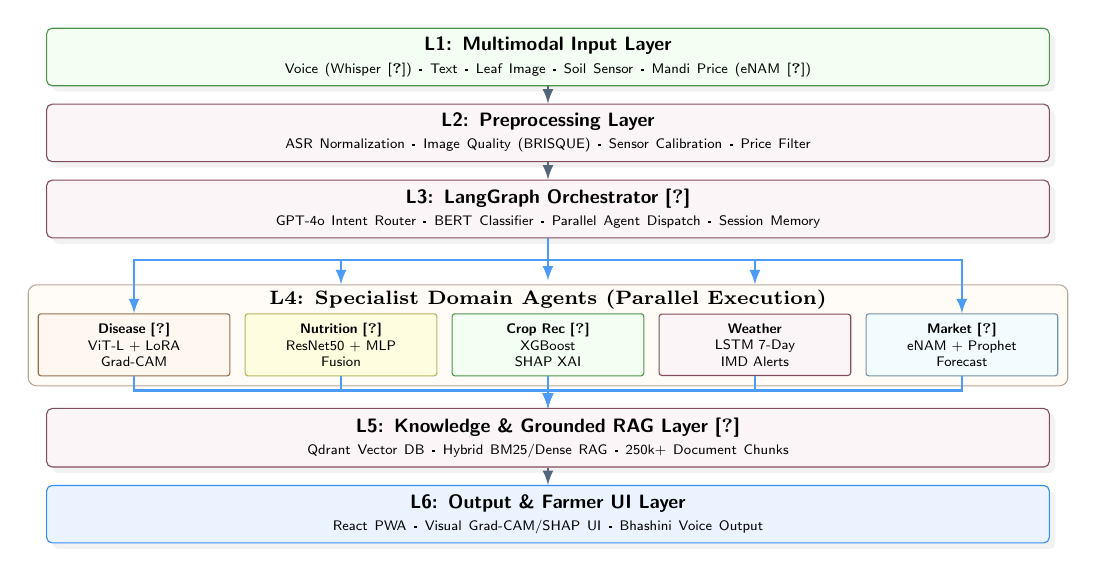
\begin{tikzpicture}[
        node distance=0.22cm and 0.18cm,
        layer/.style={rounded corners=2pt, drop shadow={opacity=0.1}, text width=12.5cm, align=center, font=\scriptsize\sffamily, minimum height=0.5cm},
        agent/.style={rounded corners=1pt, text width=2.2cm, align=center, font=\tiny\sffamily, minimum height=0.7cm}
    ]
        % Layer nodes with exact colors from HTML style
        % L1 Input: lr-t style (soft green)
        \node (l1) [layer, draw=green!40!black!70, fill=green!5!white] {\textbf{L1: Multimodal Input Layer} \\ \tiny Voice (Whisper \cite{indicAsr2025}) · Text · Leaf Image · Soil Sensor · Mandi Price (eNAM \cite{enam2023})};
        
        % L2 Preprocessing: lr-p style (soft purple/lavender)
        \node (l2) [layer, below=of l1, draw=purple!40!black!70, fill=purple!4!white] {\textbf{L2: Preprocessing Layer} \\ \tiny ASR Normalization · Image Quality (BRISQUE) · Sensor Calibration · Price Filter};
        
        % L3 Orchestrator: lr-p style (soft purple/lavender)
        \node (l3) [layer, below=of l2, draw=purple!40!black!70, fill=purple!4!white] {\textbf{L3: LangGraph Orchestrator \cite{agroaskai2024}} \\ \tiny GPT-4o Intent Router · BERT Classifier · Parallel Agent Dispatch · Session Memory};
        
        % Agent Layer (L4)
        \node (a3) [agent, below=0.95cm of l3, draw=green!40!black!70, fill=green!5!white] {\textbf{Crop Rec \cite{xaiCrop2024}}\\ XGBoost \\ SHAP XAI};
        \node (a2) [agent, left=of a3, draw=yellow!60!black!80, fill=yellow!12!white] {\textbf{Nutrition \cite{cropibot2026}}\\ ResNet50 + MLP \\ Fusion};
        \node (a1) [agent, left=of a2, draw=orange!40!black!70, fill=orange!6!white] {\textbf{Disease \cite{llmiCdp2025}}\\ ViT-L + LoRA \\ Grad-CAM};
        \node (a4) [agent, right=of a3, draw=purple!40!black!70, fill=purple!4!white] {\textbf{Weather}\\ LSTM 7-Day \\ IMD Alerts};
        \node (a5) [agent, right=of a4, draw=cyan!40!black!70, fill=cyan!5!white] {\textbf{Market \cite{enam2023}}\\ eNAM + Prophet \\ Forecast};
        
        % Group agents under L4 container box (using backgrounds and fit)
        \begin{scope}[on background layer]
            \coordinate (a3_top) at ([yshift=0.24cm]a3.north);
            \node[draw=orange!30!black!40, fill=orange!3!white, rounded corners=3pt, inner sep=0.12cm, fit=(a1) (a5) (a3_top)] (l4_container) {};
        \end{scope}

        % L4 label node drawn slightly above the container at the top center
        \node[font=\scriptsize\bfseries\color{black}, anchor=north, yshift=0.05cm] (l4_title) at (l4_container.north) {L4: Specialist Domain Agents (Parallel Execution)};
        
        % L5 Knowledge + RAG: lr-p style (soft lavender) - increased gap to 0.40cm
        \node (l5) [layer, below=0.40cm of a3, draw=purple!40!black!70, fill=purple!4!white] {\textbf{L5: Knowledge \& Grounded RAG Layer \cite{ragMaize2026}} \\ \tiny Qdrant Vector DB · Hybrid BM25/Dense RAG · 250k+ Document Chunks};
        
        % L6 Output: lr-b style (soft blue)
        \node (l6) [layer, below=of l5, draw=secondaryBlue!80, fill=secondaryBlue!8!white] {\textbf{L6: Output \& Farmer UI Layer} \\ \tiny React PWA · Visual Grad-CAM/SHAP UI · Bhashini Voice Output};
        
        % Connective arrows
        \draw[-latex, thick, primaryBlue!70] (l1) -- (l2);
        \draw[-latex, thick, primaryBlue!70] (l2) -- (l3);
        
        % Multiple branching arrows from L3 to all agents (with 2nd, 3rd, and 4th arrows terminating at the top edge/title to avoid text overlap)
        \draw[-latex, thick, secondaryBlue!70] (l3.south) -- +(0,-0.27) -| (a1.north);
        \draw[-latex, thick, secondaryBlue!70] (l3.south) -- +(0,-0.27) -| (l4_container.north -| a2.north);
        \draw[-latex, thick, secondaryBlue!70] (l3.south) -- (l4_title.north);
        \draw[-latex, thick, secondaryBlue!70] (l3.south) -- +(0,-0.27) -| (l4_container.north -| a4.north);
        \draw[-latex, thick, secondaryBlue!70] (l3.south) -- +(0,-0.27) -| (a5.north);
        
        % Multiple branching arrows from agents to L5
        \draw[-latex, thick, secondaryBlue!70] (a1.south) -- +(0,-0.18) -| (l5.north);
        \draw[-latex, thick, secondaryBlue!70] (a2.south) -- +(0,-0.18) -| (l5.north);
        \draw[-latex, thick, secondaryBlue!70] (a3.south) -- (l5.north);
        \draw[-latex, thick, secondaryBlue!70] (a4.south) -- +(0,-0.18) -| (l5.north);
        \draw[-latex, thick, secondaryBlue!70] (a5.south) -- +(0,-0.18) -| (l5.north);
        
        \draw[-latex, thick, primaryBlue!70] (l5) -- (l6);
    \end{tikzpicture}
\end{frame}


% Frame 8: Implementation Architecture
\section{Implementation Architecture}
\begin{frame}{Implementation Architecture}
    \vspace*{-0.55cm}
    \centering
    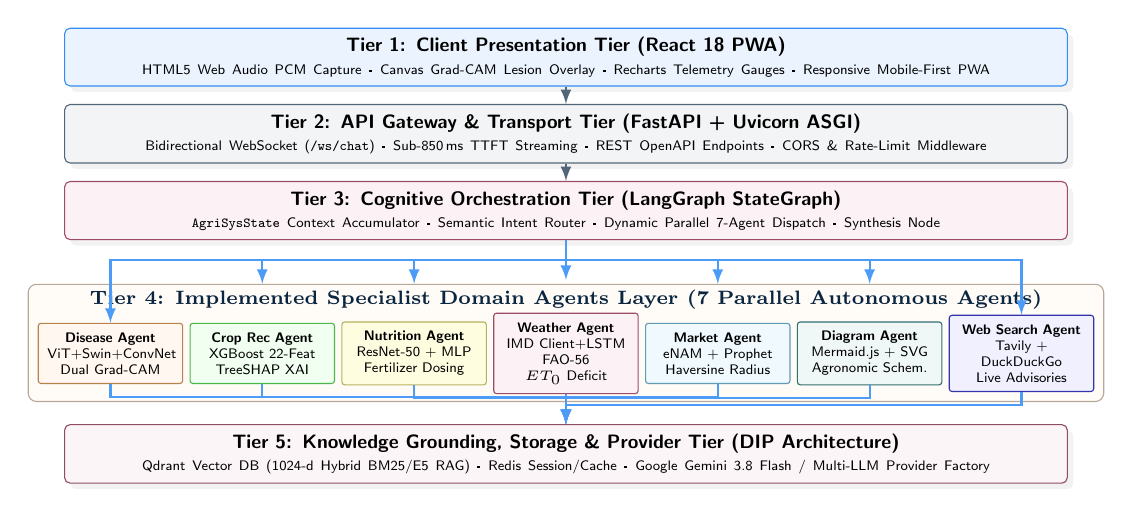
\begin{tikzpicture}[
        node distance=0.22cm and 0.18cm,
        layer/.style={rounded corners=2pt, drop shadow={opacity=0.1}, text width=12.5cm, align=center, font=\scriptsize\sffamily, minimum height=0.52cm},
        agent/.style={rounded corners=1pt, text width=1.60cm, align=center, font=\fontsize{4.8}{5.8}\selectfont\sffamily, minimum height=0.72cm}
    ]
        % T1: Client Presentation Tier
        \node (t1) [layer, draw=secondaryBlue!80, fill=secondaryBlue!8!white] {
            \textbf{Tier 1: Client Presentation Tier (React 18 PWA)} \\
            \tiny HTML5 Web Audio PCM Capture · Canvas Grad-CAM Lesion Overlay · Recharts Telemetry Gauges · Responsive Mobile-First PWA
        };

        % T2: API Gateway Tier
        \node (t2) [layer, below=of t1, draw=primaryBlue!70, fill=primaryBlue!5!white] {
            \textbf{Tier 2: API Gateway \& Transport Tier (FastAPI + Uvicorn ASGI)} \\
            \tiny Bidirectional WebSocket (\texttt{/ws/chat}) · Sub-850\,ms TTFT Streaming · REST OpenAPI Endpoints · CORS \& Rate-Limit Middleware
        };

        % T3: Cognitive Orchestration Tier
        \node (t3) [layer, below=of t2, draw=purple!60!black!70, fill=purple!5!white] {
            \textbf{Tier 3: Cognitive Orchestration Tier (LangGraph StateGraph)} \\
            \tiny \texttt{AgriSysState} Context Accumulator · Semantic Intent Router · Dynamic Parallel 7-Agent Dispatch · Synthesis Node
        };

        % T4: Specialist Domain Agents (7 Implemented Agents)
        \node (a4) [agent, below=0.92cm of t3, draw=purple!60!black!70, fill=purple!5!white] {\textbf{Weather Agent}\\IMD Client+LSTM\\FAO-56 $ET_0$ Deficit};
        \node (a3) [agent, left=0.08cm of a4, draw=yellow!60!black!80, fill=yellow!12!white] {\textbf{Nutrition Agent}\\ResNet-50 + MLP\\Fertilizer Dosing};
        \node (a2) [agent, left=0.08cm of a3, draw=green!60!black!70, fill=green!6!white] {\textbf{Crop Rec Agent}\\XGBoost 22-Feat\\TreeSHAP XAI};
        \node (a1) [agent, left=0.08cm of a2, draw=orange!60!black!70, fill=orange!6!white] {\textbf{Disease Agent}\\ViT+Swin+ConvNet\\Dual Grad-CAM};
        \node (a5) [agent, right=0.08cm of a4, draw=cyan!60!black!80, fill=cyan!6!white] {\textbf{Market Agent}\\eNAM + Prophet\\Haversine Radius};
        \node (a6) [agent, right=0.08cm of a5, draw=teal!60!black!80, fill=teal!6!white] {\textbf{Diagram Agent}\\Mermaid.js + SVG\\Agronomic Schem.};
        \node (a7) [agent, right=0.08cm of a6, draw=blue!60!black!80, fill=blue!6!white] {\textbf{Web Search Agent}\\Tavily + DuckDuckGo\\Live Advisories};

        % Container for agents
        \begin{scope}[on background layer]
            \coordinate (a4_top) at ([yshift=0.24cm]a4.north);
            \node[draw=orange!30!black!40, fill=orange!3!white, rounded corners=3pt, inner sep=0.12cm, fit=(a1) (a7) (a4_top)] (agents_container) {};
        \end{scope}
        \node[font=\scriptsize\bfseries\color{primaryBlue}, anchor=north, yshift=0.05cm] (agents_title) at (agents_container.north) {Tier 4: Implemented Specialist Domain Agents Layer (7 Parallel Autonomous Agents)};

        % T5: Knowledge, Storage & Provider Tier
        \node (t5) [layer, below=0.38cm of a4, draw=purple!50!black!70, fill=purple!4!white] {
            \textbf{Tier 5: Knowledge Grounding, Storage \& Provider Tier (DIP Architecture)} \\
            \tiny Qdrant Vector DB (1024-d Hybrid BM25/E5 RAG) · Redis Session/Cache · Google Gemini 3.8 Flash / Multi-LLM Provider Factory
        };

        % Connective Arrows
        \draw[-latex, thick, primaryBlue!70] (t1) -- (t2);
        \draw[-latex, thick, primaryBlue!70] (t2) -- (t3);

        % Branching arrows from T3 to agents
        \draw[-latex, thick, secondaryBlue!70] (t3.south) -- +(0,-0.25) -| (a1.north);
        \draw[-latex, thick, secondaryBlue!70] (t3.south) -- +(0,-0.25) -| (agents_container.north -| a2.north);
        \draw[-latex, thick, secondaryBlue!70] (t3.south) -- +(0,-0.25) -| (agents_container.north -| a3.north);
        \draw[-latex, thick, secondaryBlue!70] (t3.south) -- (agents_title.north);
        \draw[-latex, thick, secondaryBlue!70] (t3.south) -- +(0,-0.25) -| (agents_container.north -| a5.north);
        \draw[-latex, thick, secondaryBlue!70] (t3.south) -- +(0,-0.25) -| (agents_container.north -| a6.north);
        \draw[-latex, thick, secondaryBlue!70] (t3.south) -- +(0,-0.25) -| (a7.north);

        % Branching arrows from agents to T5
        \draw[-latex, thick, secondaryBlue!70] (a1.south) -- +(0,-0.16) -| (t5.north);
        \draw[-latex, thick, secondaryBlue!70] (a2.south) -- +(0,-0.16) -| (t5.north);
        \draw[-latex, thick, secondaryBlue!70] (a3.south) -- +(0,-0.16) -| (t5.north);
        \draw[-latex, thick, secondaryBlue!70] (a4.south) -- (t5.north);
        \draw[-latex, thick, secondaryBlue!70] (a5.south) -- +(0,-0.16) -| (t5.north);
        \draw[-latex, thick, secondaryBlue!70] (a6.south) -- +(0,-0.16) -| (t5.north);
        \draw[-latex, thick, secondaryBlue!70] (a7.south) -- +(0,-0.16) -| (t5.north);
    \end{tikzpicture}
\end{frame}


% Frame 9: Technical Implementation Details
\section{Implementation Details}
\begin{frame}{Technical Implementation Details}
    \vspace*{-0.35cm}
    \begin{columns}[T,onlytextwidth]
        % Left Column: Orchestration, Gateway & Clean Architecture
        \begin{column}{0.485\textwidth}
            \begin{block}{\footnotesize \textbf{Multi-Agent Orchestration \& Streaming Architecture}}
                \scriptsize
                \begin{itemize}\setlength{\itemsep}{2pt}\setlength{\parskip}{0pt}
                    \item \textbf{LangGraph Multi-Agent DAG:} Asynchronous state machine coordinating query dispatch across 7 specialist agents with \texttt{AgriSysState} memory.
                    \item \textbf{Real-Time WebSocket Protocol:} Bidirectional \texttt{/ws/chat} gateway delivering sub-850\,ms Time-to-First-Token (TTFT) and delta streaming.
                    \item \textbf{SOLID Provider Abstraction (DIP):} Strict decoupling via \texttt{BaseLLMProvider}; dynamically interfaces Gemini 3.8 Flash, Groq, and Ollama.
                    \item \textbf{Dynamic Diagram Agent:} Automated generation of interactive Mermaid workflows (IPM trees, crop timelines) and 2D measured SVG schematics (spacing grids, drip lines).
                \end{itemize}
            \end{block}
        \end{column}

        % Right Column: ML Models, XAI & Hybrid RAG Grounding
        \begin{column}{0.485\textwidth}
            \begin{block}{\footnotesize \textbf{Multimodal Machine Learning, XAI \& Hybrid RAG}}
                \scriptsize
                \begin{itemize}\setlength{\itemsep}{2pt}\setlength{\parskip}{0pt}
                    \item \textbf{Crop Disease Diagnosis:} Accuracy-weighted tri-model ensemble (ViT-L/16, Swin, ConvNeXt) + BRISQUE QA + PyTorch Grad-CAM lesion heatmaps.
                    \item \textbf{Crop Rec \& Nutrition Fusion:} 22-feature XGBoost with TreeSHAP; ResNet-50 + IoT soil sensor (NPK, pH) fusion MLP for fertilizer dosing.
                    \item \textbf{Market \& Web Search Agents:} eNAM/Agmarknet scraper with 7-day Prophet forecast; live Tavily/DuckDuckGo search for real-time agricultural advisories.
                    \item \textbf{Two-Stage Grounded Hybrid RAG:} Qdrant vector DB (1024-d Multilingual E5) + BM25Okapi sparse search merged via RRF ($k=60$) and Cross-Encoder reranking.
                \end{itemize}
            \end{block}
        \end{column}
    \end{columns}
\end{frame}
\end{document}
